\section{Implementation Details}
\label{sec:app_details}

\para{Student.} LoRA rank 32, $\alpha = 64$, applied to all attention and MLP projections (17.6M trainable parameters); AdamW with learning rate $10^{-4}$ and weight decay 0.01; batch size 8; 10\% warm-up followed by cosine decay; training length of $\max$(2 epochs, 100 steps); maximum sequence length 448; six validation checks per run with the best checkpoint selected by loss on the real validation set.
Generation uses at most 256 new tokens for code and math and 96 for stories.

\para{Teacher.} \teacher in bf16, temperature 1.0, top-$p$ 0.95, at most 512 new tokens. We treat outputs that do not parse, or that contain CJK characters (the teacher occasionally code-switches at $T = 1$), as format violations and discard them.

\para{Synthetic pools.} \Tabref{tab:pools} gives the yield of each pool.

\begin{table}[h]
    \centering
    \caption{Synthetic pools per seed.}
    \label{tab:pools}
    \resizebox{\textwidth}{!}{%
    \begin{tabular}{@{}lccl@{}}
        \toprule
        \textbf{Task} & \textbf{Requests} & \textbf{Usable} & \textbf{Filter} \\
        \midrule
        \codetask & 7,000 & 3,527--3,830 (51--55\%) & parses and passes the teacher's own three assertions \\
        \mathtask & 5,200 & 5,166--5,174 (99\%) & parses with a numeric final answer \\
        \creativetask & 5,200 & 5,197--5,199 ($\sim$100\%) & parses \\
        \bottomrule
    \end{tabular}
    }
\end{table}

\para{Data splits.} Only the train split of \roc (2018 release) has titles, so we carve its validation and test sets from that split.
For \gsm, accuracy uses the first 500 of the 1,319 test items and NLL uses all of them.

\para{Compute.} We used four RTX A6000 GPUs (48\,GB) shared with other jobs, with typically 5--20\,GB free per card. Student runs peaked at 9.0\,GB. The 117 runs took 9.2 worker-hours (about 2 hours of wall-clock time with up to five workers). Pool generation took about 52,000 teacher requests and 35 minutes. We used no API models.

\para{Software.} vLLM 0.30, PyTorch 2.13, transformers 5.19, PEFT 0.21, sentence-transformers, and SciPy.

\section{Deviations from the Pre-Specified Plan}
\label{sec:app_deviations}

We wrote the analysis plan before running experiments.
We made the following changes before producing any fine-tuned result reported here; pilot runs made under earlier settings were deleted and re-run.
\begin{itemize}[leftmargin=*,itemsep=0pt,topsep=0pt]
    \item {\bf Teacher: 7B $\rightarrow$ 3B.} The 7B model could not generate at useful throughput in the GPU memory available on shared cards.
    \item {\bf Student: full fine-tuning $\rightarrow$ LoRA,} with the epoch cap lowered from 3 to 2 after pilots showed validation loss reaching its minimum after about one epoch. Memory constraints forced this change.
    \item {\bf Ratio grid:} $\{0, 0.5, 1, 2, 3, 5, 10, 20, 50\} \rightarrow \{0, 1, 2, 3, 5, 10, 20, 30\}$, with \ratio{50} for math and creative writing only. The 3B teacher's code passes its own tests only about 51\% of the time, so the code pools cannot support \ratio{50}. The planned \ratio{50}-against-\ratio{10} contrast therefore became \ratio{30} against \ratio{10} for code.
    \item {\bf Real-data control sizes} matched to ratios $\{1, 3, 10, 30\}$ for math and creative writing and $\{1, 2.74\}$ for code.
    \item {\bf Generation-based evaluation on 500 test items} per task with capped output length.
    \item {\bf Ablations:} the unfiltered-code ablation was reduced to ratios 3 and 30, and we did not collect model-judge ratings of story quality.
\end{itemize}

\section{Additional Results}
\label{sec:app_results}

\begin{figure}[h]
    \centering
    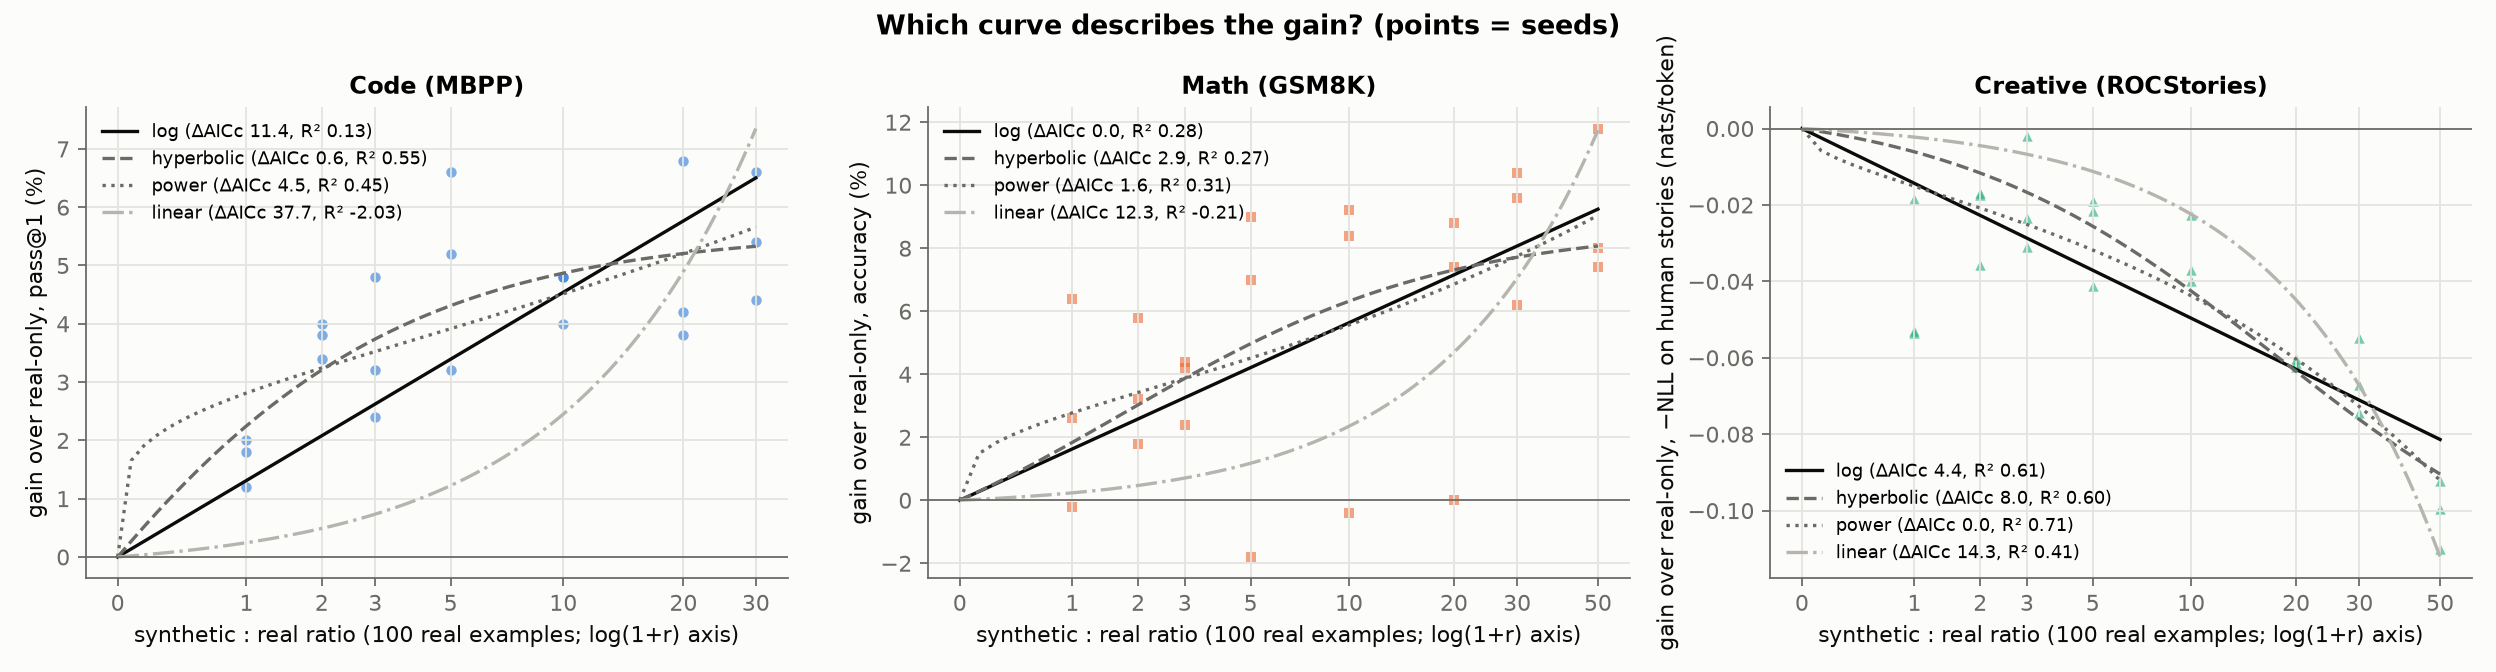
\includegraphics[width=\linewidth]{figures/curve_fits.png}
    \caption{Curve fits to seed-level gains over real-only training (points are seeds). The exponential-saturation curve is omitted because it nearly coincides with the hyperbolic one. The spread of seeds around every curve is large for code and math, which is why the fits explain little variance.}
    \label{fig:fits}
\end{figure}

\begin{table}[h]
    \centering
    \caption{Synthetic mix minus all-real control at the same training-set size, on the task metric (95\% CI; unadjusted two-sided $p$). Code and math are in accuracy points; creative writing is in $-$NLL, so negative values favor real data.}
    \label{tab:synth_real}
    \begin{tabular}{@{}llcc@{}}
        \toprule
        \textbf{Task} & \textbf{Size} & \textbf{Difference} & $p$ \\
        \midrule
        \codetask & \ratio{1} & $+1.2$ \ci{-2.1}{+4.4} & 0.424 \\
        \midrule
        \mathtask & \ratio{1} & $+2.5$ \ci{-0.8}{+5.9} & 0.138 \\
        \mathtask & \ratio{3} & $+2.6$ \ci{-0.4}{+5.4} & 0.088 \\
        \mathtask & \ratio{10} & $+3.7$ \ci{+0.4}{+7.0} & 0.030 \\
        \mathtask & \ratio{30} & $+6.5$ \ci{+2.3}{+11.0} & 0.002 \\
        \midrule
        \creativetask & \ratio{1} & $-0.058$ \ci{-0.076}{-0.037} & $<0.001$ \\
        \creativetask & \ratio{3} & $-0.072$ \ci{-0.082}{-0.060} & $<0.001$ \\
        \creativetask & \ratio{10} & $-0.116$ \ci{-0.126}{-0.108} & $<0.001$ \\
        \creativetask & \ratio{30} & $-0.173$ \ci{-0.184}{-0.161} & $<0.001$ \\
        \bottomrule
    \end{tabular}
\end{table}

\begin{table}[h]
    \centering
    \caption{Task metric per seed. Code is pass@1 (\%), math is accuracy (\%), and creative writing is NLL on human stories (nats per token).}
    \label{tab:perseed}
    \resizebox{\textwidth}{!}{%
    \begin{tabular}{@{}llccccccccc@{}}
        \toprule
        \textbf{Task} & \textbf{Seed} & 0 & \ratio{1} & \ratio{2} & \ratio{3} & \ratio{5} & \ratio{10} & \ratio{20} & \ratio{30} & \ratio{50} \\
        \midrule
        \multirow{3}{*}{\codetask} & 0 & 30.0 & 32.0 & 33.4 & 34.8 & 33.2 & 34.0 & 34.2 & 34.4 & -- \\
         & 1 & 27.4 & 28.6 & 31.2 & 29.8 & 34.0 & 32.2 & 31.2 & 32.8 & -- \\
         & 2 & 30.0 & 31.8 & 34.0 & 33.2 & 35.2 & 34.8 & 36.8 & 36.6 & -- \\
        \midrule
        \multirow{3}{*}{\mathtask} & 0 & 31.8 & 38.2 & 35.0 & 36.2 & 38.8 & 41.0 & 39.2 & 42.2 & 43.6 \\
         & 1 & 36.2 & 36.0 & 38.0 & 38.6 & 34.4 & 35.8 & 36.2 & 42.4 & 43.6 \\
         & 2 & 29.8 & 32.4 & 35.6 & 34.0 & 38.8 & 38.2 & 38.6 & 39.4 & 37.8 \\
        \midrule
        \multirow{3}{*}{\creativetask} & 0 & 2.50 & 2.55 & 2.53 & 2.52 & 2.52 & 2.54 & 2.56 & 2.55 & 2.60 \\
         & 1 & 2.50 & 2.52 & 2.52 & 2.50 & 2.52 & 2.52 & 2.56 & 2.57 & 2.59 \\
         & 2 & 2.49 & 2.54 & 2.51 & 2.52 & 2.53 & 2.53 & 2.55 & 2.56 & 2.60 \\
        \bottomrule
    \end{tabular}
    }
\end{table}

\begin{table}[h]
    \centering
    \caption{Error breakdown on \mbpp (share of test items, pooled over seeds).}
    \label{tab:errors_code}
    \resizebox{\textwidth}{!}{%
    \begin{tabular}{@{}lccccccc@{}}
        \toprule
        \textbf{Condition} & \textbf{Pass} & \textbf{Assertion} & \textbf{TypeError} & \textbf{NameError} & \textbf{SyntaxError} & \textbf{Other runtime} & \textbf{Timeout} \\
        \midrule
        Real only & 29.1\% & 55.0\% & 8.3\% & 1.8\% & 1.0\% & 4.6\% & 0.2\% \\
        \ratio{1} & 30.8\% & 53.0\% & 7.8\% & 2.2\% & 1.3\% & 4.3\% & 0.5\% \\
        \ratio{2} & 32.9\% & 54.3\% & 7.0\% & 1.6\% & 1.1\% & 2.8\% & 0.4\% \\
        \ratio{3} & 32.6\% & 54.6\% & 6.5\% & 1.7\% & 1.2\% & 2.8\% & 0.6\% \\
        \ratio{5} & 34.1\% & 52.2\% & 7.3\% & 2.0\% & 0.8\% & 3.1\% & 0.4\% \\
        \ratio{10} & 33.7\% & 53.6\% & 6.9\% & 1.0\% & 1.5\% & 3.1\% & 0.2\% \\
        \ratio{20} & 34.1\% & 52.9\% & 7.4\% & 1.3\% & 1.3\% & 2.7\% & 0.4\% \\
        \ratio{30} & 34.6\% & 51.9\% & 7.9\% & 1.7\% & 1.1\% & 2.5\% & 0.3\% \\
        \midrule
        Zero-shot student & 34.8\% & 48.0\% & 7.2\% & 2.0\% & 5.0\% & 2.8\% & 0.2\% \\
        \bottomrule
    \end{tabular}
    }
\end{table}

\begin{table}[h]
    \centering
    \caption{Error breakdown on \gsm (share of test items, pooled over seeds).}
    \label{tab:errors_math}
    \begin{tabular}{@{}lccc@{}}
        \toprule
        \textbf{Condition} & \textbf{Correct} & \textbf{Wrong answer} & \textbf{No answer line} \\
        \midrule
        Real only & 32.6\% & 66.2\% & 1.2\% \\
        \ratio{1} & 35.5\% & 62.4\% & 2.1\% \\
        \ratio{2} & 36.2\% & 58.3\% & 5.5\% \\
        \ratio{3} & 36.3\% & 60.3\% & 3.4\% \\
        \ratio{5} & 37.3\% & 59.5\% & 3.1\% \\
        \ratio{10} & 38.3\% & 57.9\% & 3.7\% \\
        \ratio{20} & 38.0\% & 58.3\% & 3.7\% \\
        \ratio{30} & 41.3\% & 56.2\% & 2.5\% \\
        \ratio{50} & 41.7\% & 54.7\% & 3.7\% \\
        \bottomrule
    \end{tabular}
\end{table}
